\documentclass[11pt]{article}
\usepackage[margin=2.5cm]{geometry}
\usepackage{tikz}
\usepackage{float} 
\usepackage{algorithm}
\usepackage{algpseudocode}
\usepackage{amsmath}
\usepackage{amssymb}
\usepackage{amsthm}
\usepackage{placeins}
\usepackage{hyperref}

% Define the 'definition' environment
\newtheorem{definition}{Definition}

\title{Segment Trees in Algorithmic Problems}
\author{Piotr Szczepaniak}
\date{\today}

\begin{document}

\maketitle

\tableofcontents

\begin{abstract}
This document provides an overview of segment trees. In the first place
We will describe some basic implementation and use case for segment trees.
Then we will try to understand the algebraic properties of segment trees for
better understanding of how they work. Finally we will dive in some more complex and not so obvious
use cases of segment trees.
\end{abstract}

\section{Foundations of Segment Trees}
Basic use case of segment tree is to store information about segments of an array.
Consider an array \(A\) with some data stored in it. To be able to perform operations on segments of this array, like
give the max value in range \(A[i, j]\) or give the sum of elements in range \(A[i, j]\), we can use a segment tree for faster
access answers to these queries. Additionally segment tree allows us to update values in the array and still be able to perform queries on segments quickly.
A segment tree is a binary tree used for storing information about segments with quick access to the data stored in it. 
To efficiently retrieve or update information about elements stored 
in segment tree we can perform various operations most common of which are
query/update on point or range.
One of the examples can be maximum value of 
elements in given range or sum of elements in given range.

\begin{figure}[H]
    \centering
    
\begin{center}
    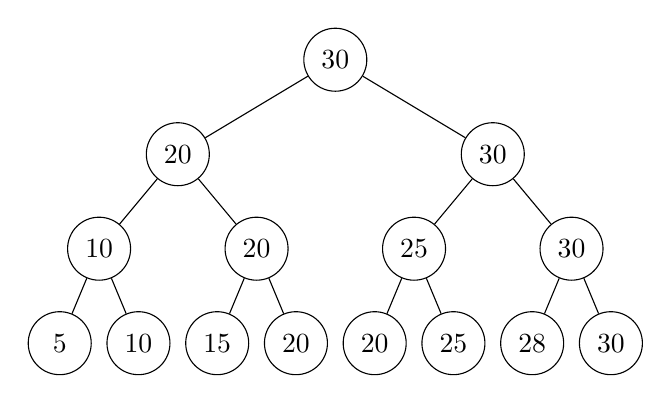
\begin{tikzpicture}[
      level distance=1.2cm,
      level 1/.style={sibling distance=4cm},
      level 2/.style={sibling distance=2cm},
      level 3/.style={sibling distance=1cm},
      every node/.style={draw,circle,minimum size=8mm,inner sep=1pt}
    ]
    
    % Root node with max value
    \node {30}
        child {node {20}
            child {node {10}
                child {node {5}}
                child {node {10}}
            }
            child {node {20}
                child {node {15}}
                child {node {20}}
            }
        }
        child {node {30}
            child {node {25}
                child {node {20}}
                child {node {25}}
            }
            child {node {30}
                child {node {28}}
                child {node {30}}
            }
        };
    
    \end{tikzpicture}
\end{center}
    \caption{Example of a segment tree with maximum value of elements in given range.}
    \label{fig:segment_tree_1}
\end{figure}

\subsection{Segment Tree with point update and range query}
To illustrate use case of segment tree we will construct tree with max value on segment.
Let's say we are given an array \(A = [5, 10, 15, 20, 30, 25, 28, 20]\) of length \(n = 8\).
For now let's assume that the input array is of size \(n = 2^{k}\) where \(k\) is integer (for different
sizes of input we will fill input array with neutral elements (see section 2) to make it's length a power of 2).
In the following implementation a segment tree is actually an array of size \(2n - 1\) where we store the whole structure.
The leaves of the tree will store the values of the array and the internal nodes will store the maximum value of the elements in their subtree.
For every internal node \(i\) the children of this node will be \(2i\) and \(2i + 1\), and the root of the tree will be at index 1.
We want to be able to perform the following operations:
\begin{itemize}
    \item \textbf{Build structure} \\
    We will create a segment tree from an array.
    To build a segment tree, we need to create a binary tree where each node will store the maximum value of elements in its subtree.
    First we copy elements of array to the leaves of the tree (as \(max(A[i, i]) = A[i]\)), then we build the tree from bottom to the top \\
    \begin{algorithm}
    \caption{Build Segment Tree for Maximum on Segment (Iterative)}
    \begin{algorithmic}
        \Procedure{BuildTree}{arr, seg}
            \For{$i = 0$ \textbf{to} $n - 1$} \Comment{Fill leaves of the segment tree}
                \State $seg[n + i] \gets A[i]$
            \EndFor
            \For{$i = n - 1$ \textbf{downto} $1$} \Comment{Calculates nodes from bottom to top}
                \State $seg[i] \gets \max(seg[2 \times i], seg[2 \times i + 1])$
            \EndFor
        \EndProcedure
    \end{algorithmic}
\end{algorithm}
    \FloatBarrier
    \item \textbf{Point update} \\
    Now let's update single value in the array and update the tree.
    We will change the value of \(A[1]\) from 10 to 35.
    To update the tree we need to change the value of the leaf node 
    and then update all the parent nodes up to the root.
    \begin{algorithm}
    \caption{Point Update on Segment Tree }
    \begin{algorithmic}
        \Procedure{update}{seg, index, value}
            \State $index \gets index + n$ \Comment{Shift index to leaf}
            \State $arr[index] \gets value$ \Comment{Update the value at the leaf}
            \While{$index > 1$} \Comment{Update the parent nodes}
                \State $index \gets \lfloor index / 2 \rfloor$
                \State $arr[index] \gets \max(arr[2 \times index], arr[2 \times index + 1])$
            \EndWhile
        \EndProcedure
    \end{algorithmic}
\end{algorithm}
    \begin{figure}[H]
        \centering
        
\begin{center}
    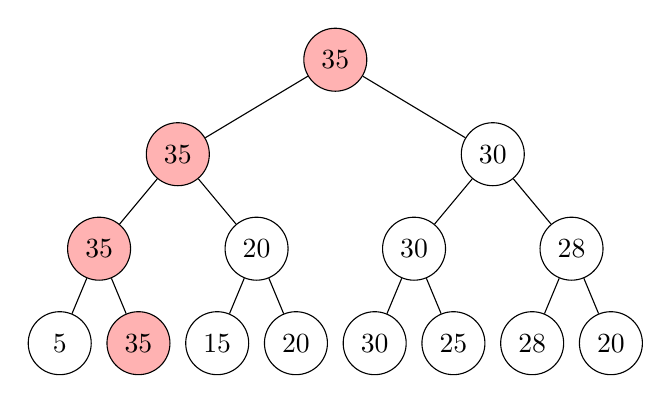
\begin{tikzpicture}[
      level distance=1.2cm,
      level 1/.style={sibling distance=4cm},
      level 2/.style={sibling distance=2cm},
      level 3/.style={sibling distance=1cm},
      every node/.style={draw,circle,minimum size=8mm,inner sep=1pt}
    ]
    
    % Root node with max value
    \node[fill=red!30] {35}
        child {node[fill=red!30] {35}
            child {node[fill=red!30] {35}
                child {node {5}}
                child {node[fill=red!30] {35}}
            }
            child {node {20}
                child {node {15}}
                child {node {20}}
            }
        }
        child {node {30}
            child {node {30}
                child {node {30}}
                child {node {25}}
            }
            child {node {28}
                child {node {28}}
                child {node {20}}
            }
        };
    
    \end{tikzpicture}
\end{center}

        \caption{Example of point update.}
        \label{fig:segment_tree_2}
    \end{figure}

    \item \textbf{Range query} \\
    Now let's say we want to find the maximum value in some range.
    To do this we need to traverse the tree from the root to the leaves and 
    find nodes that are in the range (which means that every leaf in the subtree of this node is in the range of the query). 
    Then we will get max the values of these nodes to get the final result.

    \begin{algorithm}
    \caption{Range Maximum Query on Segment Tree (Recursive, Close-Open Range)}
    \begin{algorithmic}[1]
        \Procedure{RangeQuery}{seg, index, l, r, a, b}
            \Comment{index: current node index in seg}
            \Comment{[l, r): segment represented by current node}
            \Comment{[a, b): query range}
            \If{$b \le l$ \textbf{or} $r \le a$}
                \State \Return $-\infty$ \Comment{No overlap}
            \ElsIf{$a \le l$ \textbf{and} $r \le b$}
                \State \Return $seg[index]$ \Comment{Total overlap}
            \Else
                \State $mid \gets \left\lfloor \frac{l + r}{2} \right\rfloor$
                \State $left \gets$ \Call{RangeQuery}{seg, $2 \cdot index$, $l$, $mid$, $a$, $b$}
                \State $right \gets$ \Call{RangeQuery}{seg, $2 \cdot index + 1$, $mid$, $r$, $a$, $b$}
                \State \Return $\max(left, right)$
            \EndIf
        \EndProcedure
    \end{algorithmic}
\end{algorithm}

    \begin{figure}[H]
        \centering
        
\begin{center}
    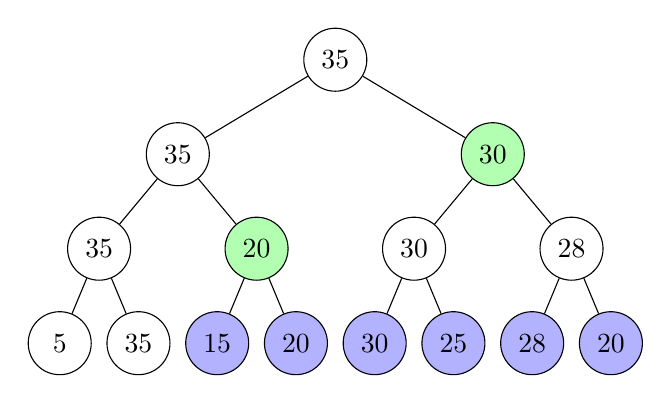
\begin{tikzpicture}[
      level distance=1.2cm,
      level 1/.style={sibling distance=4cm},
      level 2/.style={sibling distance=2cm},
      level 3/.style={sibling distance=1cm},
      every node/.style={draw,circle,minimum size=8mm,inner sep=1pt}
    ]
    
    % Root node with max value
    \node {35}
        child {node {35}
            child {node {35}
                child {node {5}}
                child {node {35}}
            }
            child {node[fill=green!30] {20}
                child {node[fill=blue!30]  {15}}
                child {node[fill=blue!30]  {20}}
            }
        }
        child {node[fill=green!30]  {30}
            child {node {30}
                child {node[fill=blue!30]  {30}}
                child {node[fill=blue!30]  {25}}
            }
            child {node  {28}
                child {node[fill=blue!30]  {28}}
                child {node[fill=blue!30] {20}}
            }
        };
    
    \end{tikzpicture}
\end{center}

        \caption{Example of range query. Blue leaves represents subarray \(A[2:7]\). Green nodes 
        are the nodes that totally overlap, red ones that don't overlap and yellow ones that partially overlap (are called in recursion).}
        \label{fig:segment_tree_3}
    \end{figure}

\end{itemize}

\subsection{Segment Tree with range update and point query}
This type of segment tree is very similar to previous one but in this case we will be able
to perform updates on given range and ask what is the value of an array at given index.
In the update operation we will update all elements in the range by adding some value to them
and in the query operation we will ask for the value of the array at given index.
The difference from the previous example is that in the nodes of the tree don't keep the
actual values of the array but some value that modifies the value from array. 
Let's take example where we add value to all elements of array on the given range. 
If the node has value $x$ it means that we added $x$ to all elements in the range of this node.
So in order to get the value of the array at given index we need to traverse the tree 
from the leaf to the root and sum all values of the nodes we passed.

\begin{itemize}
    \item \textbf{Build structure} \\
    To create a tree we only copy elements of the array to the leaves of the tree, 
    because there are no updates yet.
    \FloatBarrier
    \item \textbf{Range update} \\
    Here we want to add some given value $x$ to all elements in the range $A[a:b]$.
    This operation is similar to the range query from previous tree but here instead of
    returning the maximum value we will update the value of the node.
    \begin{algorithm}
    \caption{Range Update on Segment Tree (Recursive, Close-Open Range)}
    \begin{algorithmic}[1]
        \Procedure{RangeQuery}{seg, index, l, r, a, b, x}
            \If{$b \leq l$ \textbf{or} $r \leq a$}
                \State \Return
            \ElsIf{$a \leq l$ \textbf{and} $r \leq b$}
                \State $seg[index] \gets seg[index] + x$
            \Else
                \State $mid \gets \left\lfloor \frac{l + r}{2} \right\rfloor$
                \State \Call{RangeQuery}{seg, $2 \cdot index$, $l$, $mid$, $a$, $b$, $x$}
                \State \Call{RangeQuery}{seg, $2 \cdot index + 1$, $mid$, $r$, $a$, $b$, $x$}
                \State \Return
            \EndIf
        \EndProcedure
    \end{algorithmic}
\end{algorithm}
    \begin{figure}[H]
        \centering
        
\begin{center}
    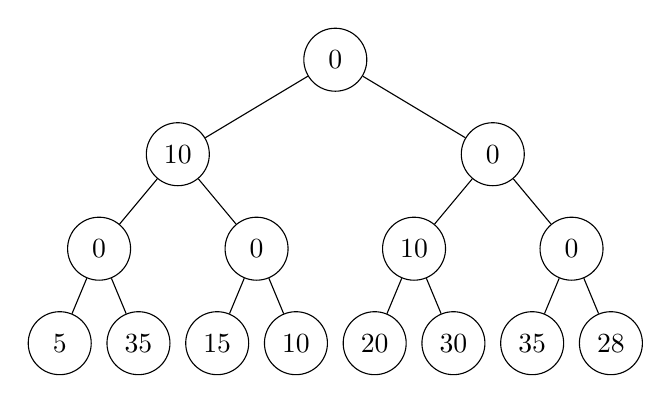
\begin{tikzpicture}[
      level distance=1.2cm,
      level 1/.style={sibling distance=4cm},
      level 2/.style={sibling distance=2cm},
      level 3/.style={sibling distance=1cm},
      every node/.style={draw,circle,minimum size=8mm,inner sep=1pt}
    ]
    
    % Root node with max value
    \node {0}
        child {node {10}
            child {node {0}
                child {node {5}}
                child {node {35}}
            }
            child {node {0}
                child {node {15}}
                child {node {10}}
            }
        }
        child {node {0}
            child {node {10}
                child {node {20}}
                child {node {30}}
            }
            child {node {0}
                child {node {35}}
                child {node {28}}
            }
        };
    
    \end{tikzpicture}
\end{center}

        \caption{Example of range update. This is a state of the tree for initial array $A = [5, 35, 15, 10, 20, 30, 25, 28]$ after range update on range $A[0:6]$ by adding value 10.}
    \end{figure}

    \item \textbf{Point query} \\
    Let's consider what is stored in the nodes of the segment tree and how to retrieve the value of the array at a given index \( i \).
    When we perform updates that affect the position \( i \), we add values to the nodes along the path from the corresponding leaf to the root. Each leaf node represents a modifier applied to the neutral element \( 0 \).
    The result of a point query at index \( i \) is the sum of all the values stored in the nodes along the path from the leaf representing \( i \) up to the root. This sum represents the combined effect of all updates (modifiers) applied to the neutral element \( 0 \) along that path.
    We use an iterative approach to perform this query because a recursive solution would be more complex.
    \begin{algorithm}
    \caption{Point Query on Segment Tree }
    \begin{algorithmic}
        \Procedure{query}{seg, index}
            \State $index \gets index + n$ \Comment{Shift index to leaf}
            \State $result \gets 0$ \Comment{Initialize result with the neutral value}
            \While{$index \geq 1$} 
                \State $result \gets result + arr[index]$
                \State $index \gets \lfloor index / 2 \rfloor$
            \EndWhile
        \EndProcedure
    \end{algorithmic}
\end{algorithm}

    If we for example ask for the value at index 0 of the array after the update visualized in
    the tree above, we will get the value 15. \\
\end{itemize}

\subsection{Segment Tree with Range Update and Range Query}

The range update, range query tree is actually a combination of two previous types of tree.
In this version we will be able to update a range of elements by adding a specified value to all elements within that range, and we can also retrieve the maximum value over a specified range.
For this tree in nodes we need to store a value (like in the 1.1 section) and modifiers (like in the 1.2 section).


\begin{itemize}
    \item \textbf{Build Structure} \\
    We need to initialize the values (max on subtree) and modifiers (neutral for now). \\
    \begin{algorithm}
    \caption{Build Segment Tree for Sum on Segment (Iterative)}
    \begin{algorithmic}
        \Procedure{BuildTree}{arr, seg}
            \For{$i = 0$ \textbf{to} $n - 1$} \Comment{Fill leaves of the segment tree}
                \State $seg[n + i] \gets \{A[i], 0\}$ \Comment{second value is for lazy propagation}
            \EndFor
            \For{$i = n - 1$ \textbf{downto} $1$} \Comment{Calculates nodes from bottom to top}
                \State $seg[i] \gets \{\max(seg[2 \times i], seg[2 \times i + 1]), 0\}$
            \EndFor
        \EndProcedure
    \end{algorithmic}
\end{algorithm} \\

    \item \textbf{Range Update} \\
    When we find the node fully in given range we update the modifier and also add the value to the node's maximum value.
    Going back from the recursion we have to update the maximum value of the node based on its children, as the update may have changed the maximum value of the subtree.
    \begin{algorithm}
    \caption{Range Update on Segment Tree }
    \begin{algorithmic}
        \Procedure{QueryUpdate}{seg, lazy index, l, r, a, b, value} \Comment{Value: value we wanted to add to each element in array}
            \State $size = r - l + 1$
            \If{$b < l$ \textbf{or} $a > r$}
                \State \Return
            \ElsIf{$a \leq l$ \textbf{and} $r \leq b$}
                \State $seg[index] \gets {seg[index] + value*size}$
                \State $lazy[index] \gets {lazy[index] + value}$
                \State \Return
            \Else
                \State $seg[index*2] \gets {seg[index*2] + value*size}$ \Comment{Update left child}
                \State $lazy[index*2] \gets {lazy[index*2] + value}$ \Comment{Push lazy to left child}
                \State $seg[index*2+1] \gets {seg[index*2+1] + value*size}$ \Comment{Same to right}
                \State $lazy[index*2+1] \gets {lazy[index*2+1] + value}$ 
                \State $lazy[index] \gets {0}$ \Comment{Reset lazy value for current node}
                \State $mid \gets \left\lfloor \frac{l + r}{2} \right\rfloor$
                \State $left \gets$ \Call{QueryUpdate}{seg, $2 \cdot index$, $l$, $mid$, $a$, $b$, $value$}
                \State $right \gets$ \Call{QueryUpdate}{seg, $2 \cdot index + 1$, $mid + 1$, $r$, $a$, $b$, $value$}
                \State $seg[index] \gets {seg[index*2] + seg[index*2+1] + lazy[index]*size}$ \Comment{Update current node after lazy propagation}
            \EndIf
        \EndProcedure
    \end{algorithmic}
\end{algorithm} \\

    \FloatBarrier

    For example, consider updating the range \( A[0:5] \) by adding 10 to each element, where the initial array is \( A = [5, 10, 15, 20, 30, 25, 20, 20] \).

    \begin{figure}[H]
        \centering
        
\begin{center}
    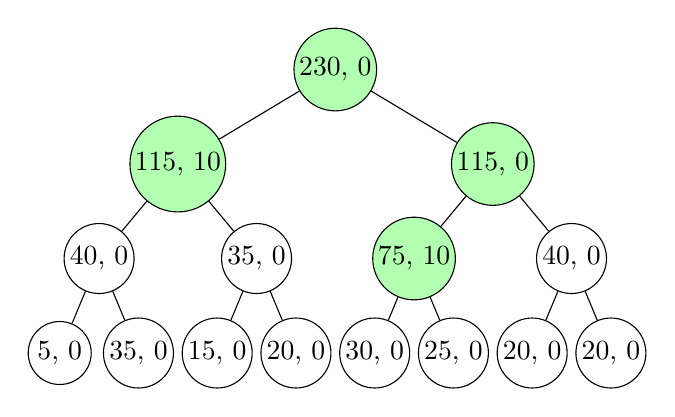
\begin{tikzpicture}[
      level distance=1.2cm,
      level 1/.style={sibling distance=4cm},
      level 2/.style={sibling distance=2cm},
      level 3/.style={sibling distance=1cm},
      every node/.style={draw,circle,minimum size=8mm,inner sep=1pt}
    ]
    
    % Root node with max value
    \node[fill=green!30] {230, 0}
        child {node[fill=green!30] {115, 10}
            child {node {40, 0}
                child {node {5, 0}}
                child {node {35, 0}}
            }
            child {node {35, 0}
                child {node  {15, 0}}
                child {node {20, 0}}
            }
        }
        child {node[fill=green!30] {115, 0}
            child {node[fill=green!30] {75, 10}
                child {node {30, 0}}
                child {node {25, 0}}
            }
            child {node  {40, 0}
                child {node {20, 0}}
                child {node {20, 0}}
            }
        };
    
    \end{tikzpicture}
\end{center}

        \caption{State of the tree after the range update. Green nodes indicate segments changed during the update.}
        \label{fig:segment_tree_4}
    \end{figure}

    \item \textbf{Range Maximum Query} \\
    To retrieve the maximum value over a specified range, the query algorithm traverses tree the same way as the update algorithm.
    As we go deeper in recursion we have to consider all modifiers on the way. This is a similar situation like in point query in section 1.2 however this time we traverse the tree top to bottom.
    \begin{algorithm}[H]
    \caption{Range Query on Segment Tree for Max with Modifiers}
    \begin{algorithmic}
        \Procedure{RangeQuery}{seg, index, l, r, a, b}
            \If{$b \leq l$ \textbf{or} $r \leq a$}
                \State \Return $-\infty$
            \EndIf
            \If{$a \leq l$ \textbf{and} $r \leq b$}
                \State \Return $seg[index].val$
            \EndIf
            \State $mid \gets \left\lfloor \frac{l + r}{2} \right\rfloor$
            \State $left \gets$ \Call{RangeQuery}{seg, $2 \cdot index$, $l$, $mid$, $a$, $b$}
            \State $right \gets$ \Call{RangeQuery}{seg, $2 \cdot index + 1$, $mid$, $r$, $a$, $b$}
            \State \Return $\max(left, right) + seg[index].mod$
        \EndProcedure
    \end{algorithmic}
\end{algorithm}


    \begin{figure}[H]
        \centering
        
\begin{center}
    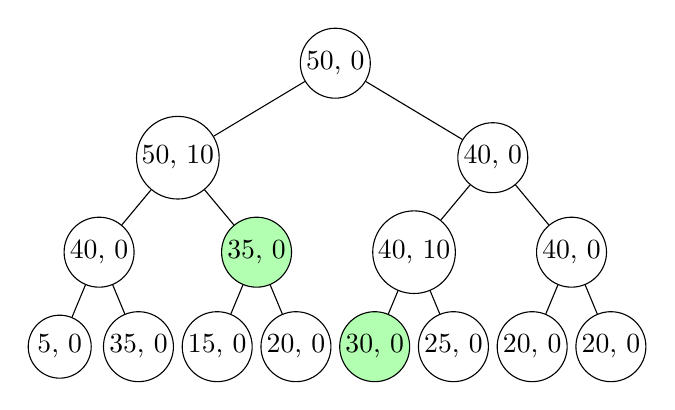
\begin{tikzpicture}[
      level distance=1.2cm,
      level 1/.style={sibling distance=4cm},
      level 2/.style={sibling distance=2cm},
      level 3/.style={sibling distance=1cm},
      every node/.style={draw,circle,minimum size=8mm,inner sep=1pt}
    ]
    
    % Root node with max value
    \node {50, 0}
        child {node {50, 10}
            child {node {40, 0}
                child {node {5, 0}}
                child {node {35, 0}}
            }
            child {node [fill=green!30] {35, 0}
                child {node  {15, 0}}
                child {node {20, 0}}
            }
        }
        child {node {40, 0}
            child {node {40, 10}
                child {node [fill=green!30] {30, 0}}
                child {node {25, 0}}
            }
            child {node  {40, 0}
                child {node {20, 0}}
                child {node {20, 0}}
            }
        };
    
    \end{tikzpicture}
\end{center}

        \caption{State of the tree after the range maximum query on the range [2:4]. Green nodes indicate those contributing to the query result. The result of the query is 45.}
        \label{fig:segment_tree_5}
    \end{figure}

\end{itemize}

\subsection{Segment Tree with Non-Comutative Update and Lazy Propagation}

The segment tree structure we have described so far works correctly for updates that are commutative and associative --- for example, adding a value to all elements of a range or querying the maximum on a range. In these cases, the order in which we apply updates does not affect the final result.

However, this approach fails if we attempt to apply non-commutative or more complex operations (such as assignment of values). The main reason is that modifiers may no longer combine in a well-defined way, and the final value would depend on the order of updates.

To support such operations, we will introduce \textbf{lazy propagation}.
In order to keep the right order of operations (when updateing) we will move the modifier to the children when traversing the tree.
This means that we will not apply the modifier immediately, but rather apply it later when we need to access the children of the node.




\vspace{1em}

\noindent Below we provide a version of the \texttt{Push} procedure that applies the modifier from a parent node to its children:

\begin{algorithm}[H]
    \caption{Push Operation for Lazy Propagation (Range Max with Assignment as Example)}
    \begin{algorithmic}
        \Procedure{Push}{seg, index}
            \If{$seg[index].active = true $} \Comment{if modifier is not empty}
                \State $seg[2 \cdot index].val \gets seg[index].mod$
                \State $seg[2 \cdot index].mod \gets  seg[index].mod$
                \State $seg[2 \cdot index + 1].val \gets  seg[index].mod$
                \State $seg[2 \cdot index + 1].mod \gets  seg[index].mod$
                \State $seg[2 \cdot index].active \gets false$
            \EndIf
        \EndProcedure
    \end{algorithmic}
\end{algorithm}

\noindent
This \texttt{Push} method ensures that before accessing or updating children, any pending modification is first applied to them, and the current node's modifier is cleared. The actual implementation of \texttt{Push} will depend on the type of operation (e.g., addition, assignment, minimum constraint).
This operation should be put right before the recursive calls in the range update.

\vspace{1em}


\section{A mathematical approach to segment trees}
In this section I will present how segment trees work from a mathematical point of view.
In order to do this we will need to understand some basic algebra that is used in segment trees.


\subsection{Monoids}
A monoid \( (S, \oplus, e) \) is a set equipped with an associative binary operation \( S \times S \to S \) and
an identity element \(e\). 
\begin{itemize}
    \item \textbf{Associativity} \\
    For all \( a, b, c \in S \), \( (a \oplus b) \oplus c = a \oplus (b \oplus c) \).
    \item \textbf{Identity element} \\
    There exists an element \( e \in S \) such that for all \( a \in S \), \( a \oplus e = e \oplus a = a \).
    \item \textbf{Commutativity} \\
    Monoid is called \textbf{commutative} if for all \( a, b \in S \), \( a \oplus b = b \oplus a \).
\end{itemize}
Examples of monoids:
\begin{itemize}
    \item \textbf{Natural numbers under addition, (\(\mathbb{N}\), +, 0) } \\
    In this simple example we can see that addition is associative and commutative. 
    Adding 0 (neutral element) to any of the numbers will not change the result of the operation.
    \item \textbf{Strings over an alphabet, (\(\Sigma^*\), \(\cdot\), \(\epsilon\))} \\
    \(\Sigma^*\) - set of all strings over an alphabet \(\Sigma\) \\
    \(\cdot\) - concatenation of strings \\
    \(\epsilon\) - empty string \\
    This is a example of non-commutative monoid. Concatenation of strings is associative but not commutative as we can see in the following example.
    \begin{equation}
        \text{abc} \cdot \text{def} = \text{abcdef} \neq \text{defabc} = \text{def} \cdot \text{abc}
    \end{equation}
\end{itemize}

\subsection{Application of Monoids to Segment Trees}
How does this all relate to segment trees?
First of all we can see that segment trees requires the properties of monoids to work.
The associativity of the operation is required to be able to combine the results of the operations on the segments.
The identity element is required when we ask for the result of the operation on an empty segment or 
when we want extend our initial array to a power of 2. 
Since all segment trees must preserve monoid properties, we can think more generic 
approach to the implementation. We will create a generic segment tree that can be used for any monoid for 
range queries and point updates. Let \(\oplus\) be a binary operation on a monoid \(S\) and let \(e\) be the identity element of the monoid.

\begin{algorithm}
    \caption{Segment Tree over a Monoid \((S, \ast, e)\)}
    \begin{algorithmic}[1]
        \Procedure{BuildTree}{$A$, $seg$, $e$}
            \State $n \gets$ next power of two greater than or equal to $|A|$
            \For{$i = 0$ \textbf{to} $|A| - 1$}
                \State $seg[n + i] \gets A[i]$ \Comment{Insert original values}
            \EndFor
            \For{$i = |A|$ \textbf{to} $n - 1$}
                \State $seg[n + i] \gets e$ \Comment{Pad remaining leaves with identity}
            \EndFor
            \For{$i = n - 1$ \textbf{downto} $1$}
                \State $seg[i] \gets seg[2 \times i] \ast seg[2 \times i + 1]$
            \EndFor
        \EndProcedure

        \\
        
        \Procedure{Update}{$arr$, $index$, $value$}
            \State $index \gets index + n$ \Comment{Move to the leaf node}
            \State $arr[index] \gets value$ \Comment{Set the new value at the leaf}
            \While{$index > 1$}
                \State $index \gets \lfloor index / 2 \rfloor$ \Comment{Move to parent}
                \State $arr[index] \gets arr[2 \times index] \ast arr[2 \times index + 1]$
            \EndWhile
        \EndProcedure

        \\

        \Procedure{RangeQuery}{$seg$, $index$, $l$, $r$, $a$, $b$, $e$}
        \Comment{$index$: current node in segment tree}
        \Comment{$[l, r]$: range covered by node}
        \Comment{$[a, b]$: query range}
        \If{$b \leq l$ \textbf{or} $r \leq a$}
            \State \Return $e$ \Comment{No overlap}
        \ElsIf{$a \leq l$ \textbf{and} $r \leq b$}
            \State \Return $seg[index]$ \Comment{Total overlap}
        \Else
            \State $mid \gets \left\lfloor \frac{l + r}{2} \right\rfloor$
            \State $left \gets$ \Call{RangeQuery}{$seg$, $2 \cdot index$, $l$, $mid$, $a$, $b$, $e$}
            \State $right \gets$ \Call{RangeQuery}{$seg$, $2 \cdot index + 1$, $mid$, $r$, $a$, $b$, $e$}
            \State \Return $left \ast right$
        \EndIf
    \EndProcedure
    \end{algorithmic}
\end{algorithm}
\FloatBarrier
Now we can replace this generic monoid with some specific one.
For example we can use a segment tree for sum of elements in given range.
In this case we will use \(\oplus\) as addition and \(e\) as 0. 
Another example can be a segment tree for maximum value in given range.
In this case we will use \(\oplus\) as maximum and \(e\) as \(-\infty\).
We can see that using this generic approach we can create a segment tree for any monoid.

\subsection{Homomorphism}
A homomorphism is a structure-preserving map between two algebraic structures.
In this section we will look at homomorphisms between monoids.
Let \( (S, \oplus, e) \) and \( (T, \cdot, \theta) \) be two monoids.
A function \( f: S \to T \) is a homomorphism if:
\begin{itemize}
    \item \textbf{Preserves the operation} \\
    For all \( a, b \in S \), \( f(a \oplus b) = f(a) \cdot f(b) \).
\end{itemize}
Let's consider a simple example of homomorphism between two monoids.
Let \( S = (\mathbb{N}, +, 0) \) and \( T = (\mathbb{N}, \cdot, 1) \).
Let \( f: S \to T \) be defined as \( f(x) = 2^x \).
We can see that:
\begin{itemize}
    \item \( f(a + b) = 2^{a + b} = 2^a \cdot 2^b = f(a) \cdot f(b) \)
    \item \( f(0) = 2^0 = 1 \)
\end{itemize}

\subsection{Endomorphism}

A special case of a homomorphism is an \emph{endomorphism}.  
An endomorphism is a homomorphism from a monoid to itself.

Let us consider a simple example of an endomorphism.  
Let \( S = (\mathbb{N}, +, 0) \) be the monoid of natural numbers under addition.  
Define \( f: S \to S \) by \( f(x) = 2x \).

We can verify that \( f \) is a homomorphism by checking:
\[
    f(a + b) = 2(a + b) = 2a + 2b = f(a) + f(b)
\]

An interesting property of endomorphisms is that the set of all endomorphisms of a monoid forms a monoid itself.

Let \( E \) be the set of all endomorphisms of the monoid \( S \).  
We define a binary operation \( \oplus \) on \( E \) by composition:
\[
    (f \oplus g)(x) = f(g(x))
\]

This operation is associative, and the identity element is the identity endomorphism \( e \) defined by \( e(x) = x \).  
Hence, \( (E, \oplus, e) \) is a monoid.

\subsection{Application of Endomorphisms to Segment Trees}
In this section we will implement a generic segment tree for range update and range query.
The operations in the segment tree are now defined over a monoid \( (S, \oplus, e) \) and we will use an endomorphism \( f: S \to S \) to modify the values in the segment tree.


\begin{algorithm}[H]
    \caption{Range Update on Segment Tree over value Monoid and modifier Monoid }
    \begin{algorithmic}[1]
        \Procedure{RangeUpdate}{seg, index, l, r, a, b, $f$}
            \If{$b \le l$ \textbf{or} $r \le a$}
                \State \Return
            \ElsIf{$a \le l$ \textbf{and} $r \le b$}
                \State $seg[index].val \gets f(seg[index].val)$
                \State $seg[index].mod \gets f \circ seg[index].mod$ \Comment{Keep in mind the order of operations}
                \State \Return
            \Else
                \State $mid \gets \lfloor (l + r)/2 \rfloor$
                \State \Call{RangeUpdate}{seg, $2 \cdot index$, $l$, $mid$, $a$, $b$, f}
                \State \Call{RangeUpdate}{seg, $2 \cdot index + 1$, $mid$, $r$, $a$, $b$, f}
                \State \Call{Pull}{seg, index}
            \EndIf
        \EndProcedure

        \\

        \Procedure{RangeQuery}{seg, index, l, r, a, b}
            \If{$b \le l$ \textbf{or} $r \le a$}
                \State \Return $e$
            \ElsIf{$a \le l$ \textbf{and} $r \le b$}
                \State \Return $seg[index].val$
            \Else
                \State $mid \gets \lfloor (l + r)/2 \rfloor$
                \State $left \gets$ \Call{RangeQuery}{seg, $2 \cdot index$, $l$, $mid$, $a$, $b$}
                \State $right \gets$ \Call{RangeQuery}{seg, $2 \cdot index + 1$, $mid$, $r$, $a$, $b$}
                \State \Return $f(left \oplus right)$ 
            \EndIf
        \EndProcedure

        \\

        \Procedure{Pull}{seg, index}
            \State $seg[index].val \gets seg[index].mod\big(seg[2 \cdot index].val \oplus seg[2 \cdot index + 1].val\big)$
        \EndProcedure


    \\

    \Procedure{Push}{seg, index}
        \State $seg[2 \cdot index].val \gets seg[index].mod(seg[2 \cdot index].val) $
        \State $seg[2 \cdot index].mod \gets  seg[index].mod \circ seg[2 \cdot index].mod$
        \State $seg[2 \cdot index + 1].val \gets  seg[index].mod(seg[2 \cdot index + 1].val) $
        \State $seg[2 \cdot index + 1].mod \gets  seg[index].mod \circ seg[2 \cdot index + 1].mod$
        \State $seg[2 \cdot index].mod \gets id$ \Comment{Reset the modifier}
    \EndProcedure
    \end{algorithmic}
\end{algorithm}

\vspace{0.1cm}
\FloatBarrier
Using this generic approach we can simply replace the monoid with some specific one and
set endomorphism as some function that we want to apply to the range of elements.

\subsection{Examples of Monoids and Operations for Segment Trees}

Here are some practical examples of monoids and operations suitable for segment trees with range updates and queries:

\begin{enumerate}
    \item \textbf{Change values on a range, get minimum on a range} \\
    \begin{itemize}
        \item Value monoid: \( (S, \oplus, e) = (\mathbb{Z}, \min, +\infty) \) — stores the minimum value on a segment.
        \item Modifier monoid: \( (M, \star, \mathrm{id}) = (\mathbb{Z} \cup \{\bot\}, \text{overwrite}, \bot) \) — assigns a value to the whole segment.
        \item Apply function: 
        \[
            f(x) = \begin{cases}
            f & \text{if } f \neq \bot \\
            x & \text{if } f = \bot
            \end{cases}
        \]
    \end{itemize}

    \item \textbf{Add a string to all elements in the array, get the string with the most letters 'a' in a range} \\
    \begin{itemize}
        \item Value monoid: \( (S, \oplus, e) = (\text{Strings}, \max_a, "") \), where \(\max_a\) returns the string with the highest count of letter 'a'.
        \item Modifier monoid: \( (M, \star, \mathrm{id}) = (\text{Strings}, \text{concatenate}, "") \) — concatenates strings as updates.
        \item Apply function: 
        \[
            f(x) = x \text{ concatenated with } f
        \]
    \end{itemize}

    \item \textbf{Range updates with addition, query maximum prefix sum on a range} \\
    \begin{itemize}
        \item Value monoid: \( S = \{ \text{max prefix sum, total sum} \} \) with operation combining prefix sums properly.
        \item Modifier monoid: \( (M, \star, \mathrm{id}) = (\mathbb{Z}, +, 0) \) — add values to elements.
        \item Apply function: 
        \[
            f(x) = \text{update prefix sums and total sums by adding } f
        \]
    \end{itemize}
\end{enumerate}

\textit{Note:} The exact structure and merge rules of complex monoids (like prefix sums or strings) need to be carefully defined to maintain associativity and identity elements.


\section{Binsearch on Segment Tree}
In this section we will see that we can use segment trees not only for queries and updates but also for
binary search. Let's consider the following problem:
\begin{center}
    \textit{Given an array $a[1 \ldots n]$, answer a query $Q(i, j, x)$: What is the smallest index $k$ so that $a[k] \geq x$ in subarray  $a[i \ldots j]$?}\\[1ex]
\end{center}

We want to be able to answer this query in \(O(\log{n})\) time. We can create 
a segment tree with max value in given range but this is not enough. We need to upgrade our segment tree
with binsearch operation, which goes as follows:
\begin{itemize}
    \item Traverse recursively the tree to find the nodes that are in the range of the query (just like in range query). Always go to the left child first.
    \item For every nodes perform a binary search on the subtree.
    \item Binsearch 
        \begin{itemize}
            \item if right child's value is less than x, return -1 (no such index)
            \item if left child's value is greater than x, go to left child
            \item else go to right child
        \end{itemize}
    \item Because we traverse the tree from left to right, we can be sure that the first binsearch that returns index different than -1 is the answer to the query.
    \item if no such index was found, return -1.
\end{itemize}

\begin{algorithm}
    \caption{Find First Index With Value Greater Than $x$ in Range $[a, b)$}
    \begin{algorithmic}[1]
        \Procedure{Query}{segTree, index, l, r, a, b, x}
            \Comment{index: current node index}
            \Comment{[l, r): segment represented by current node}
            \Comment{[a, b): query range}
            \If{$b \leq l$ \textbf{or} $r \leq a$}
                \State \Return $-1$ \Comment{No overlap}
            \ElsIf{$a \leq l$ \textbf{and} $r \leq b$}
                \State \Return \Call{BinarySearch}{segTree, index, x}
            \Else
                \State $mid \gets \left\lfloor \frac{l + r}{2} \right\rfloor$
                \State $left \gets$ \Call{Query}{segTree, $2 \cdot index$, $l$, $mid$, $a$, $b$, $x$}
                \If{$left \neq -1$}
                    \State \Return $left$
                \EndIf
                \State \Return \Call{Query}{segTree, $2 \cdot index + 1$, $mid$, $r$, $a$, $b$, $x$}
            \EndIf
        \EndProcedure
        \\
        \Procedure{BinarySearch}{tree, index, x}
            \While{$index*2 < tree.size$}
                \State $left \gets tree[index * 2]$
                \If{$left > x$}
                    \State $index \gets index * 2$
                \Else
                    \State $index \gets index * 2 + 1$
                \EndIf
            \EndWhile
            \If{$tree[index] > x$}
                \State \Return $index$
            \Else
                \State \Return $-1$ \Comment{No index found}
            \EndIf
        \EndProcedure
    \end{algorithmic}
\end{algorithm}

\FloatBarrier
Let's consider the following example: \\
We have an array \(A = [5, 8, 2, 7, 1, 11, 13, 12, 19, 14, 15, 0, 15, 10, 15, 4]\) and we want to find the smallest index \(k\) such that \(A[k] \geq 14\) in the range \(A[5:12]\).

\begin{figure}[H]
    \centering
    
\begin{center}
    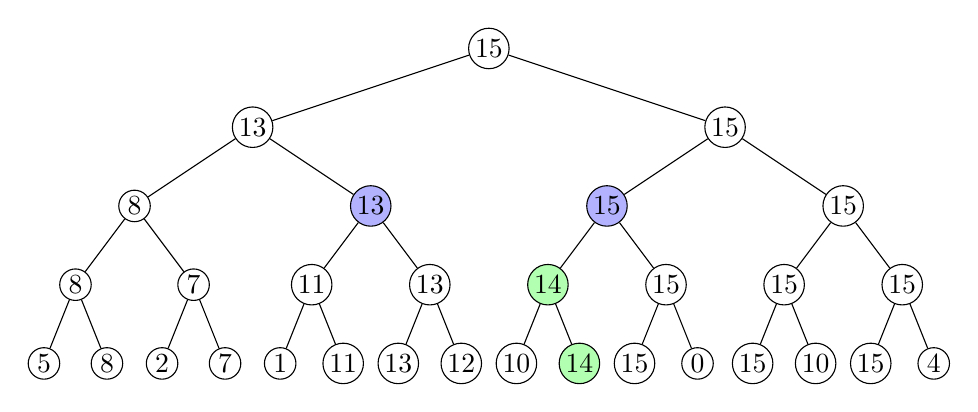
\begin{tikzpicture}[
        level distance=1cm,
        sibling distance=0pt,
        every node/.style = {circle, draw, minimum size=4mm, inner sep=1pt},
        level 1/.style={sibling distance=6cm},
        level 2/.style={sibling distance=3cm},
        level 3/.style={sibling distance=1.5cm},
        level 4/.style={sibling distance=0.8cm},
        level 5/.style={sibling distance=0.5cm}
      ]
      
      \node {15}
      child {node {13}
        child {node {8}
          child {node {8}
            child {node {5}}
            child {node {8}}
          }
          child {node {7}
            child {node {2}}
            child {node {7}}
          }
        }
        child {node[fill=blue!30] {13}
          child {node {11}
            child {node {1}}
            child {node {11}}
          }
          child {node {13}
            child {node {13}}
            child {node {12}}
          }
        }
      }
      child {node {15}
        child {node[fill=blue!30] {15}
          child {node[fill=green!30] {14}
            child {node {10}}
            child {node[fill=green!30] {14}}
          }
          child {node {15}
            child {node {15}}
            child {node {0}}
          }
        }
        child {node {15}
          child {node {15}
            child {node {15}}
            child {node {10}}
          }
          child {node {15}
            child {node {15}}
            child {node {4}}
          }
        }
      };
      
      \end{tikzpicture}
\end{center}

    \caption{The blue nodes are the ones that we performed binsearch on. The green nodes are the ones that binsearch traversed. The result of the query is index 10. As we can see, the first binsearch (on node with value 13 returned -1)}
    \label{fig:segment_tree_1}
\end{figure}

\end{document}